
\section{Methods}

\subsection{Data Generation}
\label{subsec:data_generation}


The large-scale simulation datasets required to train the \gls{ml} models are generated by solvating solutes in a water box, equilibrating them, and propagating the system over time. Both coordinates and forces are extracted from these representative trajectories specifically to facilitate the force-matching scheme detailed in the Methods section.


The data pipeline is designed for large-scale simulation of amino acid sequences. 

The pipeline begins with the generation of three-dimensional solute structures from amino acid sequences using AmberTools \texttt{tleap}, which produces capped or uncapped PDB files depending on the desired terminus configuration. 
These structures are subsequently solvated in a TIP3P explicit water box using OpenMM's \texttt{Modeller}, with a padding around the solute to ensure a sufficiently large solvation shell. The AMBER14 force field is applied to parameterize all interactions. Prior to production, each system undergoes energy minimization followed by an NPT equilibration phase. The replicas are propagated simultaneously using Langevin dynamics. The solute position and forces are logged to npz files. The entire workflow from sequence input to job submission is orchestrated by a pipeline script that constructs SLURM batch jobs and submits them to the cluster, enabling the parallel processing of many sequences.

\begin{figure}
    \centering
    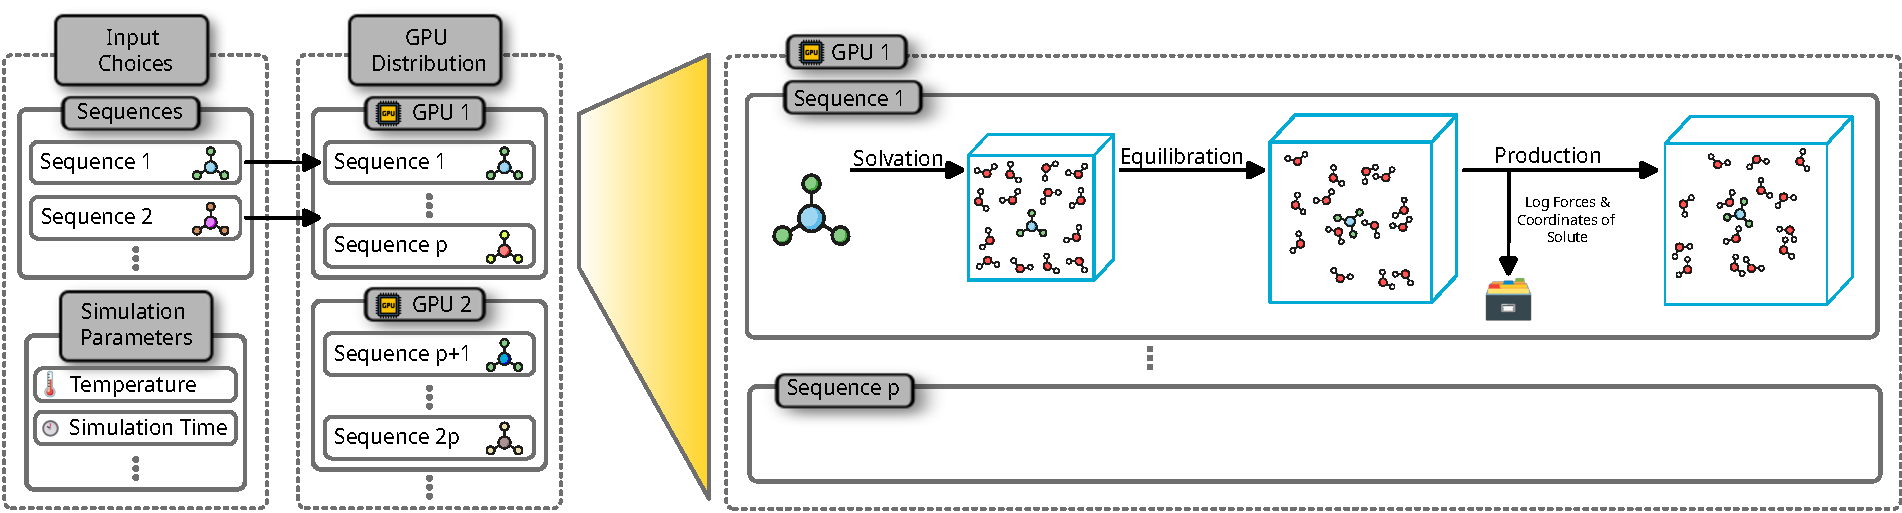
\includegraphics[width=1\linewidth]{images/data_pipeline_framework.pdf}
    \caption{Caption}
    \label{fig:placeholder}
\end{figure}


\subsection{Datasets}
\label{subsec:production_datasets}

The data for this paper was generated using the parameters detailed in Table~\ref{tab:production_datasets}. For all datasets, the temperature was maintained at 300\,K, with a padding of 1.2\,nm, both NPT and NVT equilibration phases lasted 100\,ns, and 2,000,000 frames were generated.

\begin{table*}[htbp]
    \centering
    \begin{tabular}{l r r}
        \toprule
        \textbf{Dataset} & \textbf{Number of Peptides} & \textbf{Simulation Time} \\
        \midrule
        Dipeptides (Train) & 280 & 1\,\textmu s \\
        Dipeptides (Test) & 120 & 1\,\textmu s \\
        Tetrapeptides (Train) & 1,500 & 500\,ns \\
        Tetrapeptides (Test) & 30 & 5\,\textmu s \\
        \bottomrule
    \end{tabular}
    \caption{Overview of simulation parameters, phase durations, and sequence composition across all primary dataset partitions.}
    \label{tab:production_datasets}
\end{table*}


To generate the tetrapeptide datasets, we used a permutation method inspired by \cite{tan2025amortized} to ensure a perfectly balanced frequency of all 20 standard amino acids.

We generated the sequences by building a base string of evenly distributed amino acids, randomly shuffling it, and cutting it into adjacent blocks of four. For the test set (30 tetrapeptides), this initial string contained exactly 6 copies of each amino acid. For the training set (1,500 tetrapeptides), it contained exactly 300 copies of each.

The simulation is a sequential algorithm mainly scaling in the number of atoms in the system. The number of atoms in the explicitly solvated system scales quadratically to the number of atoms in the molecule or the length of the sequence. Using a vacuum model in which the effects of the solvent are not computed explicitly thus scales only linearly in the number of atoms in the peptide / sequence length.
% Thus using a ML model, which estimates the effects of the water may be more efficient.



\subsection{Coarse-Graining}
\label{cg}

Coarse-graining (CG) is a widely used approach in MD simulations that reduces computational complexity by approximating groups of atoms as single effective particles, known as CG beads \citep{cgInBioSims}. The interactions between CG beads are described by a CG energy function, which is parameterized to reproduce the behavior of the underlying all-atom system. By simulating these CG beads instead of all individual atoms, one can efficiently approximate the dynamics and thermodynamics of complex molecular systems \citep{cgReviewNoid}. In general, we seek to approximate the potential of mean force (PMF) with the CG energy function. The PMF allows for sampling from the CG space \citep{schopmansEtAl}.

Consider a molecular system with \(N\) atoms and atomic coordinates \(\mathbf{r} \in \mathbb{R}^{3N}\). The CG mapping \(\xi: \mathbb{R}^{3N} \to \mathbb{R}^{3n}\) reduces the degrees of freedom by projecting \(\mathbf{r}\) into a lower-dimensional space $\mathbf{x}=\xi(\mathbf{r})$ with $n<N$. The parameters $\theta$ of the CG model define the CG energy function $V(\mathbf{x}; \theta)$. In classical CG approaches, these include physical parameters such as force constants and partial charges, whereas in ML-based CG, they correspond to the weights of a neural network \citep{cgBasics}. A common objective is to have the equilibrium distribution of the CG system approximate the equilibrium distribution of the all-atom system being mapped to the CG space. This is called thermodynamic consistency and can be achieved by enforcing 
\begin{align}
    V(\mathbf{x}, \theta) \equiv -k_B T \,\text{ln} \, p^{\text{CG}}(\mathbf{x}) + \text{const} \, ,
\end{align}
where $k_B$ is the Boltzmann constant, $T$ the temperature, and $p^{\text{CG}}(\mathbf{x})$ is the mapped equilibrium distribution of the atomic coordinates described by
\begin{align}
    p^{\text{CG}}(\mathbf{x)} = \frac{\int \mu (\mathbf{r}) \delta(x - \xi(\mathbf{r})) \text{d}\mathbf{r}}{\int \mu (\mathbf{r}) \text{d} \mathbf{r}}
\end{align}
with Dirac delta function $\delta$ and Boltzmann distribution $\mu$ \citep{cgBasics}.

In a solute-solvent system with solute coordinates $\mathbf{y}$ and solvent coordinates $\mathbf{w}$, implicit solvation can be interpreted as a special case of coarse-graining, where the CG mapping is defined as
\begin{align}
    \xi\left( 
\begin{bmatrix}
\mathbf{y} \\
\mathbf{w}
\end{bmatrix}
\right) = \mathbf{y}.
\end{align}

\subsection{Force Matching}
\label{subsec:force_matching}

Our goal is to construct a parameterized potential $V_{\theta}(\mathbf{y})$ that approximates the true Potential of Mean Force (PMF) of the solute, $V_{\mathrm{PMF}}(\mathbf{y})$. This PMF serves as the effective potential governing the solute dynamics in the implicit solvent space. Following the variational force-matching formulation for coarse-grained models \citep{noid_multiscale_2008}, we define the exact PMF by integrating out the solvent degrees of freedom $\mathbf{w}$. The PMF is the conditional free energy of the solute:
\begin{align}
    V_{\mathrm{PMF}}(\mathbf{y}) &\equiv -k_B T \ln p(\mathbf{y}) + C \nonumber \\
    &= -k_B T \ln \frac{\int \mu(\mathbf{y}, \mathbf{w}) \, \mathrm{d}\mathbf{w}}{\iint \mu(\mathbf{y}, \mathbf{w}) \, \mathrm{d}\mathbf{y} \, \mathrm{d}\mathbf{w}} + C \, ,
\end{align}
where $p(\mathbf{y})$ is the marginal equilibrium probability density of the solute coordinates, obtained by integrating the joint Boltzmann distribution $\mu(\mathbf{y}, \mathbf{w})$ over the solvent coordinates $\mathbf{w}$.

Unfortunately, we cannot directly train a machine learning model to predict $V_{\mathrm{PMF}}(\mathbf{y})$ because explicit energy labels for the PMF are not available. However, we can leverage the relationship between the PMF and the all-atom forces. The negative gradient of the PMF (the mean force) is equal to the conditional expectation of the instantaneous forces projected onto the solute degrees of freedom, which can be explicitly written as an integral over the Boltzmann distribution:
\begin{align}
    -\nabla_{\mathbf{y}} V_{\mathrm{PMF}}(\mathbf{y}) &= \mathbb{E}_{(\mathbf{y}, \mathbf{w}) \sim \mu} \left[ \mathbf{f}_{\mathrm{solute}}(\mathbf{y}, \mathbf{w}) \mid \xi(\mathbf{y}, \mathbf{w}) = \mathbf{y} \right] \nonumber \\
    &= \frac{\int \mathbf{f}_{\mathrm{solute}}(\mathbf{y}, \mathbf{w}) \mu(\mathbf{y}, \mathbf{w}) \, \mathrm{d}\mathbf{w}}{\int \mu(\mathbf{y}, \mathbf{w}) \, \mathrm{d}\mathbf{w}} \, .
\end{align}
Because implicit solvation is a "slicing" CG mapping (where the solvent atoms are discarded and the solute atoms are kept exactly as they are), the projected forces $\mathbf{f}_{\mathrm{solute}}(\mathbf{y}, \mathbf{w})$ are simply the instantaneous total forces acting on the solute atoms in the explicit-solvent system.

Evaluating this conditional expectation directly is computationally intractable. Instead, the multiscale force-matching theorem demonstrates that we can optimize a surrogate loss. Minimizing the expected squared difference between the instantaneous explicit forces and the negative gradient of our model potential over the joint equilibrium distribution:
\begin{align}
    \mathcal{L}(\theta) &= \mathbb{E}_{(\mathbf{y}, \mathbf{w}) \sim \mu} \left[ \left\lVert \mathbf{f}_{\mathrm{solute}}(\mathbf{y}, \mathbf{w}) + \nabla_{\mathbf{y}} V_{\theta}(\mathbf{y}) \right\rVert_2^2 \right] \nonumber \\
    &= \frac{\iint \left\lVert \mathbf{f}_{\mathrm{solute}}(\mathbf{y}, \mathbf{w}) + \nabla_{\mathbf{y}} V_{\theta}(\mathbf{y}) \right\rVert_2^2 \mu(\mathbf{y}, \mathbf{w}) \, \mathrm{d}\mathbf{y} \, \mathrm{d}\mathbf{w}}{\iint \mu(\mathbf{y}, \mathbf{w}) \, \mathrm{d}\mathbf{y} \, \mathrm{d}\mathbf{w}}
\end{align}
variationally yields the correct PMF gradient, such that our model $V_{\theta}(\mathbf{y})$ approximates $V_{\mathrm{PMF}}(\mathbf{y})$. 

To build a highly expressive physical inductive bias \citep{machine_learning_implicit_solvation}, we define our PMF model on the solute Cartesian coordinates $\mathbf{y} \in \mathbb{R}^{3N}$ as:
\begin{align}
    V_{\theta}(\mathbf{y}) = V_{\mathrm{vac}}(\mathbf{y}) + V_{\mathrm{solv},\theta}(\mathbf{y}) \, ,
\end{align}
where $V_{\mathrm{vac}}$ is the known vacuum potential given by the classical force field, and $V_{\mathrm{solv},\theta}$ is the learned solvation free-energy term parameterized by a neural network. The corresponding total model force $\hat{\mathbf{f}}_{\theta}(\mathbf{y})$ on the solute atoms is obtained by combining two distinct differentiation methods. The classical vacuum forces, $\mathbf{f}_{\mathrm{vac}}(\mathbf{y})$, are computed efficiently using the optimized analytical derivatives of the empirical force field natively implemented in the molecular dynamics engine (here, OpenMM). In contrast, the neural network solvation forces, $\mathbf{f}_{\mathrm{solv},\theta}(\mathbf{y})$, are obtained via automatic differentiation:
\begin{align}
    \hat{\mathbf{f}}_{\theta}(\mathbf{y}) = -\nabla_{\mathbf{y}} V_{\theta}(\mathbf{y}) = \mathbf{f}_{\mathrm{vac}}(\mathbf{y}) + \mathbf{f}_{\mathrm{solv},\theta}(\mathbf{y}) \, .
\end{align}

Given a set of fine-grained training samples $\{(\mathbf{y}_i, \mathbf{f}^{\mathrm{exp}}_i)\}_{i=1}^{M}$ drawn from an explicit-solvent equilibrium trajectory, where $\mathbf{f}^{\mathrm{exp}}_i \in \mathbb{R}^{3N}$ denotes the instantaneous total force acting on the $N$ solute atoms, we transition from the theoretical expectation to the empirical force-matching loss:
\begin{align}
    \mathcal{L}_{\mathrm{FM}}(\theta) &= \frac{1}{3NM}\sum_{i=1}^{M} \left\lVert\mathbf{f}^{\mathrm{exp}}_i - \hat{\mathbf{f}}_{\theta}(\mathbf{y}_i)\right\rVert_2^2 \nonumber \\
    &= \frac{1}{3NM}\sum_{i=1}^{M} \left\lVert\mathbf{f}^{\mathrm{exp}}_i - \mathbf{f}_{\mathrm{vac}}(\mathbf{y}_i) + \nabla_{\mathbf{y}}V_{\mathrm{solv},\theta}(\mathbf{y})\big|_{\mathbf{y}=\mathbf{y}_i}\right\rVert_2^2 \, .
\end{align}
By minimizing this mean-squared error over all $3N$ Cartesian components, the neural network learns to predict the solvation energy such that the total model effectively captures the underlying PMF of the implicit solvent system.


\subsection{Model Architecture}

\subsubsection{Delta-Learning Framework}
The baseline model architecture employed in this work adapts the formulation from \cite{machine_learning_implicit_solvation}. The model incorporates a physical prior based on the AMBER \texttt{ff14SB} force field \citep{maier2015ff14sb}, which computes the baseline molecular mechanics energy of the system in vacuum. This establishes a delta-learning scheme, wherein the neural network is tasked exclusively with learning the complex solvation free-energy correction $V_{\mathrm{solv},\theta}$ of the system. The core representation learning is driven by the SchNet architecture \citep{schutt2018schnet}, a continuous-filter convolutional neural network designed to operate on atomistic graphs.

\begin{figure}[htbp]
    \centering
    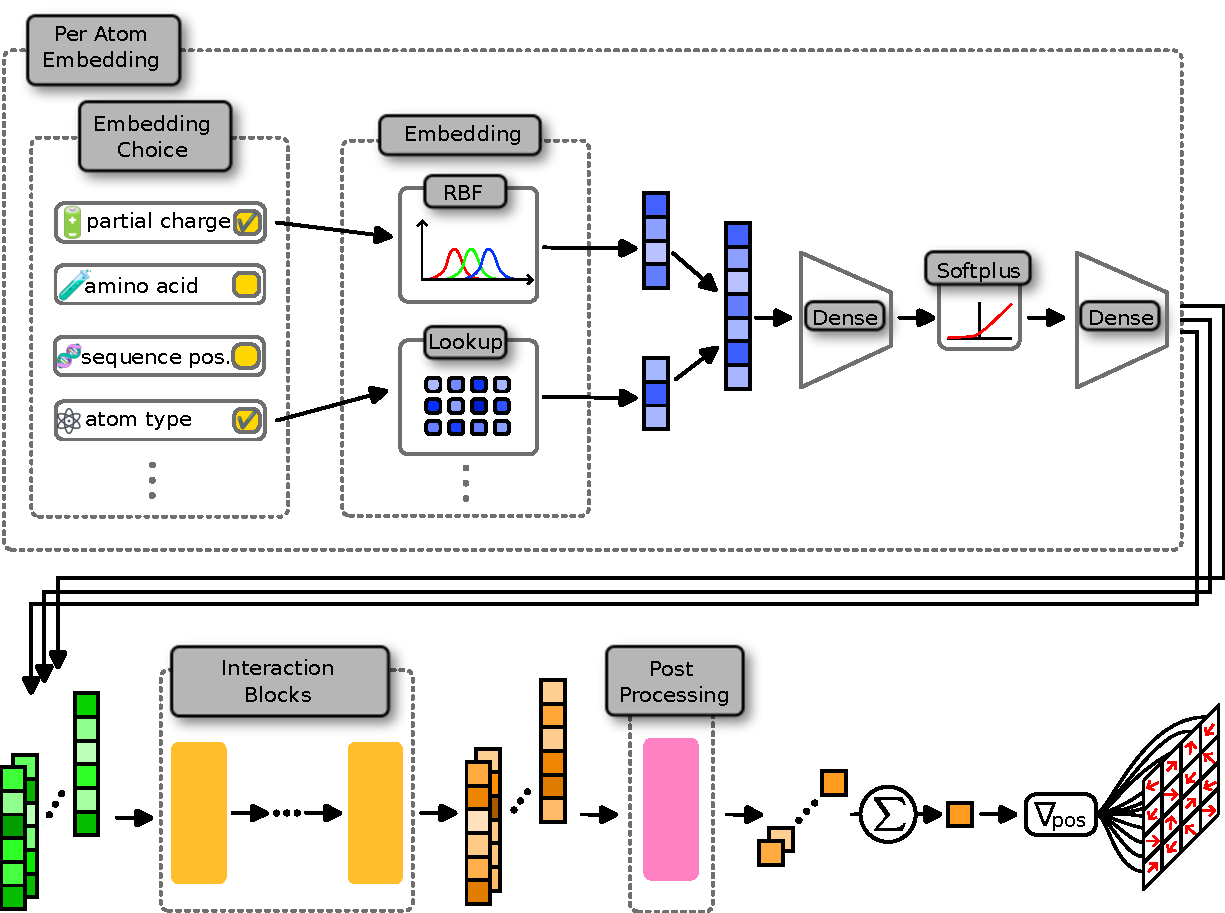
\includegraphics[width=0.9\linewidth]{images/model_architecture.pdf}
    \caption{Overview of the complete model architecture. \textbf{Top:} The dynamic embedding layer routes selected atomic descriptors to appropriate preprocessing modules, such as RBF kernels for continuous data (e.g., partial charges) or lookup tables for categorical data (e.g., atom types). These individual representations are concatenated and projected through dense neural networks to form the initial atomic embeddings. \textbf{Bottom:} The SchNet core processes these initial embeddings through a series of continuous-filter convolutional interaction blocks and post-processing layers. The outputs are summed ($\Sigma$) to predict the scalar system energy. Finally, the target atomic forces are derived by computing the gradient of the predicted energy with respect to the atomic positions ($\nabla_{\text{pos}}$).}
    \label{fig:model_architecture}
\end{figure}

\subsubsection{Modular Atomic Embeddings}
Recent studies have highlighted that the design of initial atomic embeddings is critical to overall model performance \citep{machine_learning_implicit_solvation, klein_transferable_2024}. To easily and systematically explore this impactful feature space, we employ a modular embedding architecture. Unlike the original SchNet formulation, where initial atomic embeddings are derived solely from the atomic number, our model dynamically constructs the initial atomic embedding $\mathbf{x}_i^{(0)}$ for each atom $i$ based on a flexible combination of topological and physical descriptors. As illustrated in Figure \ref{fig:model_architecture}, atomic features are routed to specific preprocessing modules depending on their mathematical domain.

For categorical features (e.g., atom types, parent amino acid identity, or sequence position), the discrete class $k_i$ is mapped to a dense, learnable vector representation via an embedding lookup:
\begin{equation}
    \mathbf{e}_i^{\mathrm{cat}} = \mathrm{Embedding}(k_i).
\end{equation}


Conversely, continuous physical node features $c_i$, such as partial charges derived from the force field, are expanded into a higher-dimensional space using a node-level Radial Basis Function (RBF) kernel. Specifically, the scalar feature $c_i$ is mapped to a dense vector $\mathbf{e}_i^{\mathrm{cont}} \in \mathbb{R}^{N_c}$ with components defined as:
\begin{equation}
    [\mathbf{e}_i^{\mathrm{cont}}]_k = \exp\left(-\gamma (c_i - \mu_k)^2\right),
\end{equation}
where $N_c$ is the number of basis functions, $\gamma$ is a hyperparameter controlling the width of the Gaussian basis, and the centers $\mu_k$ are uniformly distributed across the expected range of the feature values (e.g., $[-1, 1]$ for partial charges). Note that this expansion of node-level scalars is distinct from SchNet's standard edge-level RBF expansion of interatomic distances.

The independently processed feature vectors are concatenated and projected to the hidden dimensionality of the SchNet architecture through a dense Multi-Layer Perceptron (MLP) featuring a Shifted Softplus activation function:
\begin{equation}
    \mathbf{x}_i^{(0)} = \mathrm{MLP} \left( \big[ \mathbf{e}_i^{\mathrm{cat, 1}} \parallel \dots \parallel \mathbf{e}_i^{\mathrm{cat, M}} \parallel \mathbf{e}_i^{\mathrm{cont, 1}} \parallel \dots \parallel \mathbf{e}_i^{\mathrm{cont, N}} \big] \right),
\end{equation}
where $\parallel$ denotes the concatenation operator. This modular formulation allows for seamless ablation of input features. In this study, we systematically evaluate three representation schemes: (1) a minimal categorical encoding of the five fundamental element types (H, C, N, O, S); (2) a \textit{TBG + full} scheme \citep{klein_transferable_2024} combining 54 topological atom classes, 20 amino acid classes, and discrete sequence positions; and (3) an augmented q-ISSNet scheme integrating continuous atomic partial charges \citep{machine_learning_implicit_solvation}.

\subsubsection{Energy Prediction and Force Derivation}
Once initialized, the atomic representations $\mathbf{x}_i^{(0)}$ are iteratively updated through $L$ SchNet interaction blocks. To transform the initial embeddings into the final representations $\mathbf{x}_i^{(L)}$, the network employs continuous-filter convolutions that aggregate local neighborhood information. At each interaction layer $\ell \in \{0, \dots, L-1\}$, the representation of atom $i$ is updated via a residual connection:
\begin{equation}
    \mathbf{x}_i^{(\ell+1)} = \mathbf{x}_i^{(\ell)} + \mathbf{v}_i^{(\ell)},
\end{equation}
where the update vector $\mathbf{v}_i^{(\ell)}$ is computed by passing the input representations through an initial atom-wise linear layer, convolving them with a continuous distance filter, and processing the result through an atom-wise Multi-Layer Perceptron (MLP):
\begin{equation}
    \mathbf{v}_i^{(\ell)} = \mathrm{MLP}_{\mathrm{update}}^{(\ell)} \left( \sum_{j \neq i} \left( \mathbf{W}_{\mathrm{in}}^{(\ell)} \mathbf{x}_j^{(\ell)} \right) \circ \mathbf{W}_{\mathrm{filter}}^{(\ell)}(d_{ij}) \right).
\end{equation}
Here, $\mathbf{W}_{\mathrm{in}}^{(\ell)}$ denotes the learnable weights of the initial atom-wise linear transformation, and $\circ$ denotes element-wise multiplication. The filter-generating network $\mathbf{W}_{\mathrm{filter}}^{(\ell)}$ dynamically maps the RBF-expanded interatomic distances $d_{ij} = \lVert\mathbf{r}_i - \mathbf{r}_j\rVert_2$ to the filter weight space using a dense MLP with Shifted Softplus activations. $\mathrm{MLP}_{\mathrm{update}}^{(\ell)}$ consists of two subsequent atom-wise linear layers separated by a Shifted Softplus activation. Because these continuous-filter convolutions depend exclusively on $E(3)$-invariant distances $d_{ij}$, the intermediate states and the final hidden state $\mathbf{x}_i^{(L)}$ remain strictly invariant to global rotations and translations of the input coordinates $\mathbf{y}$.

Following the final interaction block, an atom-wise MLP maps each atom's hidden state to a scalar atomic energy contribution. These local contributions are sum-pooled to predict the total macroscopic solvation energy of the system:
\begin{equation}
    V_{\mathrm{solv},\theta}(\mathbf{y}) = \sum_{i=1}^{N} \mathrm{MLP}_{\mathrm{atom}}\left(\mathbf{x}_i^{(L)}\right).
\end{equation}
Finally, the learned solvation forces $\mathbf{f}_{\mathrm{solv},\theta}$ are derived via automatic differentiation by computing the exact negative gradient of the predicted energy with respect to the atomic positions $\mathbf{y}$:
\begin{equation}
    \mathbf{f}_{\mathrm{solv},\theta}(\mathbf{y}) = -\nabla_{\mathbf{y}} V_{\mathrm{solv},\theta}(\mathbf{y}).
\end{equation}
By taking the spatial gradient of an $E(3)$-invariant scalar energy, we mathematically guarantee that the resulting predicted forces are strictly $E(3)$-equivariant, inherently preserving the rotational and translational symmetries of the physical system prior to force-matching optimization.





\subsection{Dataset Orchestration During Training}
Training on massive molecular datasets presents significant memory constraints, as the data typically exceeds available RAM. Consequently, a sophisticated data-loading pipeline is required to prevent GPU starvation while ensuring sufficient data shuffling to mitigate catastrophic forgetting during sequential epoch iterations (todo cite this). We explored numerous data-loading strategies; approaches that were ultimately deemed unsuitable for this training pipeline are documented in Appendix (todo add link). A critical challenge in this context is concurrent dataset access by multiple GPUs, which can precipitate severe disk I/O bottlenecks if not carefully managed.

To establish the final dataset architecture, four primary challenges must be addressed. First, trajectories generated via explicit solvent simulations exhibit strong temporal correlations due to sequential logging; therefore, intra-trajectory shuffling is imperative. Second, to prevent catastrophic forgetting, the training batches must be uniformly sampled across all molecules present in the training set. Third, dataset iteration must be highly efficient, balancing the I/O operations of swapping data into RAM with the need to continuously supply the GPU with sufficient data to maximize utilization. Lastly, the dataset architecture must facilitate highly concurrent access, ensuring efficient training scalability even when multiple GPUs simultaneously operate on the shared dataset.

To resolve these issues, the dataset is orchestrated as follows: after partitioning the molecules into train, validation, and test splits, the frames for each molecule are locally shuffled. These shuffled frames are then divided into a defined number of chunks (shards $0$ to $\text{num\_shards}$). The total number of shards is calculated such that the cumulative size of a given shard index across all molecules within a split (e.g., the training set) equals a target memory footprint, $X$, specified during dataset generation. The static per-molecule metadata, which includes the embedding features detailed in Section (TODO ref), is stored in a separate hierarchical level and shared across all corresponding frames. This decoupled storage strategy facilitates the dynamic injection of new features, obviating the need for computationally expensive dataset regeneration. To optimize I/O, the resulting shards are striped across multiple disks. This enables parallelized read access, preventing the read speed of any single drive from becoming a bottleneck.

To resolve these issues, the dataset is orchestrated as follows: after partitioning the molecules into train, validation, and test splits, the frames for each molecule are locally shuffled. These shuffled frames are then divided into a defined number of chunks (shards $0$ to $N_{\text{shards}}$). The total number of shards is calculated such that the cumulative size of a given shard index across all molecules within a split (e.g., the training set) equals a target memory footprint, $X$, specified during dataset generation. The static per-molecule metadata, which includes the embedding features detailed in Section \ref{sec:model_architecture}, is stored in a separate hierarchical level and shared across all corresponding frames. This decoupled storage strategy facilitates the dynamic injection of new features, obviating the need for computationally expensive dataset regeneration. To optimize I/O, the resulting shards are striped across multiple disks. This enables parallelized read access, preventing the read speed of any single drive from becoming a bottleneck.

During training, the model accesses this information via a randomized queue that iterates over the pre-built shards. For example, loading "shard 1" entails loading the first shard of every molecule within a given split. A specialized prefetching mechanism operates in parallel to asynchronously load upcoming shards into a memory queue, from which the final training batches are constructed. By combining the randomized access patterns of separate distributed jobs with this asynchronous prefetch queue, we sustain high disk I/O throughput and maximize the computational efficiency of all participating GPUs. Furthermore, the initial intra-molecule shuffling, combined with the aggregation of molecular data during shard loading, operates on sufficiently large data partitions to approximate a global randomized access pattern, thereby effectively mitigating catastrophic forgetting.

\begin{figure}
    \centering
    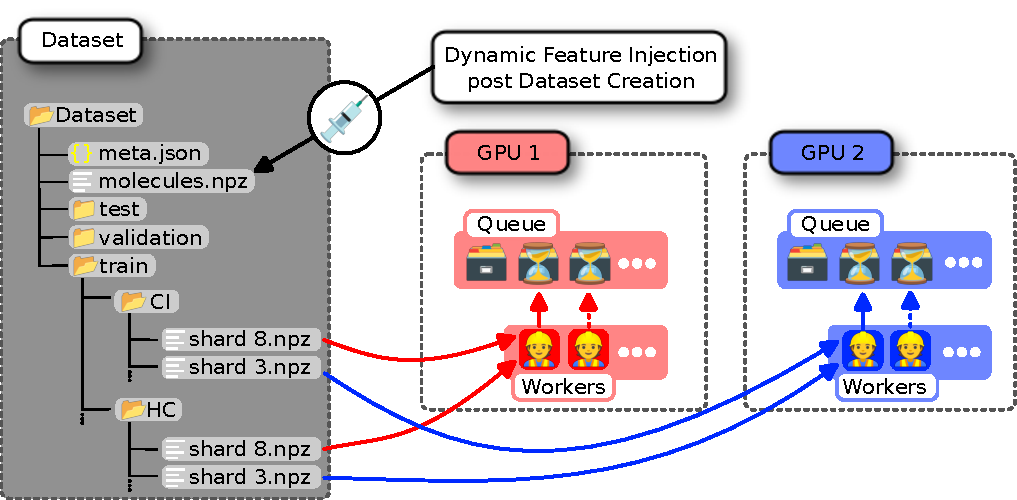
\includegraphics[width=0.7\linewidth]{images/dataset_architecture.pdf}
    \caption{Overview of the dataset architecture and concurrent data-loading pipeline. The hierarchical dataset separates static per-molecule metadata (molecules.npz) to facilitate dynamic feature injection. Frame data within the training splits (e.g., Cl, HC) are partitioned into individual shards. To maximize utilization and mitigate I/O bottlenecks during distributed training, independent workers asynchronously fetch randomized shards from the shared dataset and prefetch them into dedicated memory queues for parallel processing across multiple GPUs.}
    \label{fig:placeholder}
\end{figure}

\subsection{Simulation Framework}

To facilitate the evaluation and production deployment of the developed models, we introduced a framework built upon the Atomic Simulation Environment (ASE) (cite) that enables the parallel simulation of arbitrary PyTorch models. During molecular dynamics simulations, the primary computational bottleneck of the integration step is typically the force evaluation. The inherent batch processing capabilities of PyTorch align perfectly with parallelizing this step. 

To achieve this, multiple ASE \texttt{Atoms} objects are instantiated simultaneously. While the force computations are batched, the remainder of the integration steps are managed concurrently using threading. Initial tests utilizing standard Python threading proved highly inefficient due to the severe context-switching overhead associated with kernel-level threads. Instead, we employed green threads managed by a custom round-robin hub scheduler, which yielded a significant 10x speedup over our initial standard threading implementation.

The execution strategy is as follows: integrators are initialized as separate green threads, but yield execution to the next thread in the queue via a hook intercepted during the \texttt{Atoms} object's force call. Once an iteration completes—meaning all active threads have yielded once—a single batched GPU forward pass is issued, encompassing the atomic positions from all threaded integrators. 

\begin{figure}
    \centering
    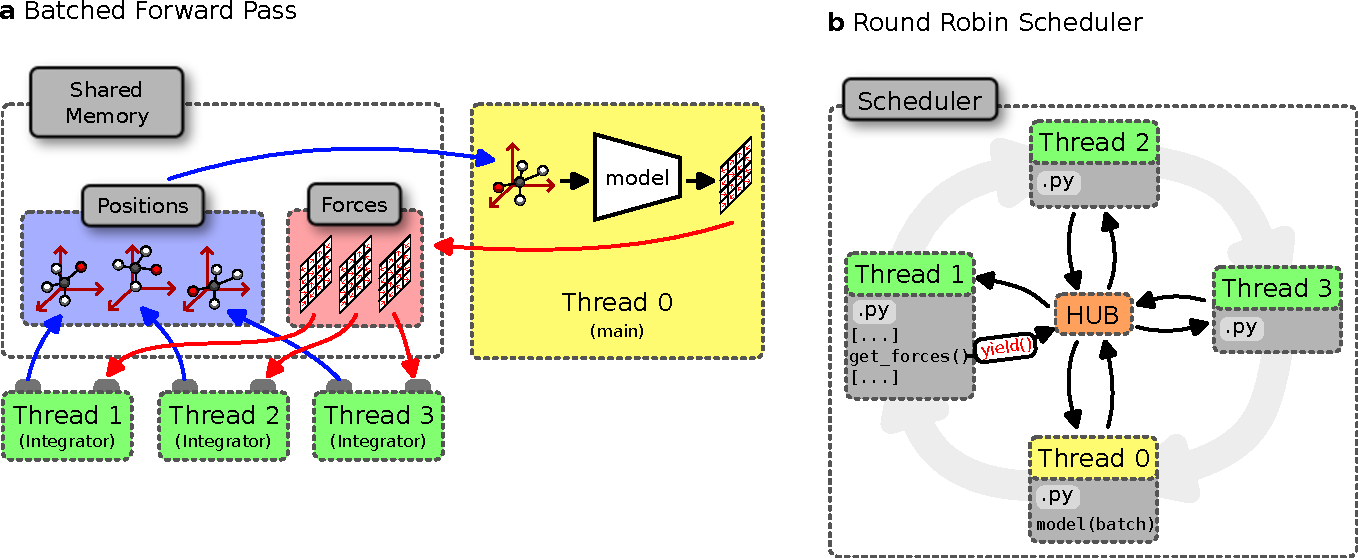
\includegraphics[width=0.5\linewidth]{images/scheduler.pdf}
    \caption{Schematic of the green-thread-based scheduling framework. Individual simulation threads (green) run sequentially and yield execution via a yield() hook during the force evaluation call (get\_forces()). The central HUB manages these yields in a round-robin fashion, aggregating atomic positions from all threads into a single batched GPU forward pass (yellow) before returning the computed forces and resuming thread execution.}
    \label{fig:placeholder}
\end{figure}

Because the parallelization is implemented via a simple hook on the force evaluation, the mechanism remains fundamentally task-agnostic. Any process relying on force evaluations can benefit from this substantial acceleration. For instance, geometric energy minimization using the BFGS algorithm can be parallelized using the exact same codebase. As shown in Figure~\ref{fig:speedup_multiatoms}, the batched scheme achieves near-linear scaling up to 128 systems (57$\times$ speedup), where GPU compute and scheduling overhead contribute equally to the total step time. Beyond this point, overhead from batching and data transfer grows superlinearly, yet a throughput gain of 79$\times$ is still realized at 2048 simultaneous systems.


\begin{figure}[htbp]
    \centering
    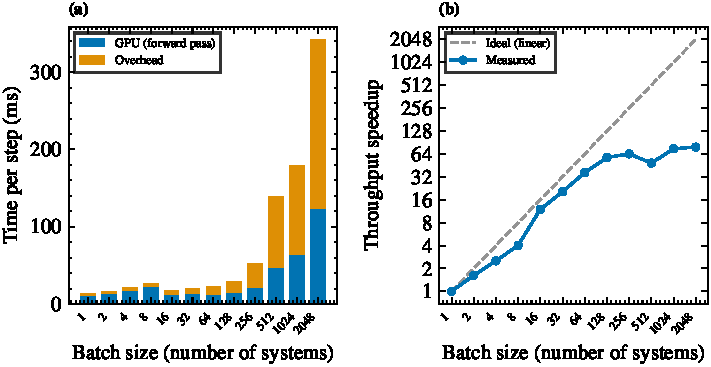
\includegraphics[width=1\linewidth]{images/multiatoms_profiling.pdf}
    \caption{Performance scaling of batched parallel MD simulations. \textbf{(a)}~Time per integration step broken down into GPU forward pass and scheduling/preprocessing overhead. \textbf{(b)}~Throughput speedup relative to a single-system baseline, compared against ideal linear scaling. Near-linear speedup is achieved up to 256 systems, beyond which overhead from batching and data transfer becomes the dominant cost.}
    \label{fig:speedup_multiatoms}
\end{figure}
